\documentclass{article}
\usepackage{graphicx} % Required for inserting images
\usepackage{svg}
\usepackage[utf8]{inputenc}
\usepackage[T1]{fontenc}
\usepackage{inconsolata}
\usepackage[portuguese]{babel}
\usepackage{listings}
\usepackage{verbatim} 
\usepackage[margin=2cm]{geometry}
\usepackage{float}
\usepackage{subfig}
\usepackage{xcolor}
\usepackage{textcomp}

% *********************************************************************

\definecolor{fnpurple}{rgb}{0.42, 0.16, 0.49}
\definecolor{fnteal}{rgb}{0.00, 0.42, 0.51}
\definecolor{fngreen}{rgb}{0.00, 0.45, 0.36}
\definecolor{fngold}{rgb}{0.65, 0.50, 0.00}
\definecolor{fnrust}{rgb}{0.71, 0.36, 0.21}
\definecolor{fnblue}{rgb}{0.34, 0.36, 0.70}
\definecolor{fncomment}{rgb}{0.5, 0.5, 0.5}


\lstdefinestyle{ocaml_light}{
    language=[Objective]Caml,
    backgroundcolor=\color{white},
    basicstyle=\ttfamily\footnotesize\color{fngold},
    keywordstyle=\color{fnpurple}\bfseries,
    commentstyle=\color{fncomment}\itshape,
    stringstyle=\color{fnrust},
    emph={None, Some, true, false, Ok, Error},
    emphstyle=\color{fnteal}\bfseries,
    emph={[2]List, Array, String, Map, Set, Option, fst, snd, failwith, raise, print_endline, Printf},
    emphstyle={[2]\color{fngreen}\bfseries},
    breakatwhitespace=false,
    breaklines=true,
    captionpos=b,
    keepspaces=true,
    numbers=none,
    showspaces=false,
    showstringspaces=false,
    showtabs=false,
    tabsize=2,
    upquote=true,
    literate=
        {:}{{\textcolor{fnblue}{:}}}1
        {=}{{\textcolor{fnblue}{=}}}1
        {[}{{\textcolor{fnblue}{[}}}1
        {]}{{\textcolor{fnblue}{]}}}1
        {(}{{\textcolor{fnblue}{(}}}1
        {)}{{\textcolor{fnblue}{)}}}1
        {\{}{{\textcolor{fnblue}{\{}}}1
        {\}}{{\textcolor{fnblue}{\}}}}1
        {|}{{\textcolor{fnblue}{|}}}1
        {;}{{\textcolor{fnblue}{;}}}1
        {->}{{\textcolor{fnblue}{->}}}2
        {::}{{\textcolor{fnblue}{::}}}2
        {-}{{\textcolor{fnblue}{-}}}1
        {+}{{\textcolor{fnblue}{+}}}1
        {*}{{\textcolor{fnblue}{*}}}1
}

% *********************************************************************



\title{Relatório BII}


\begin{document}
\author{Guilherme Guerreiro e Miguel Alvito}
\maketitle

\begin{abstract}
Trabalhos recentes propuseram novas variantes de Random Access List, a Improved e Advanced Myers List, que reduziram o número de 
travessias no pior caso, no entanto, a variante Advanced fá-lo à custa da perda da operação cons em tempo constante. Este relatório 
levanta duas questões (i) é possível recuperar o cons em tempo constante na Advanced Myers List removendo as restrições impostas? (ii) é possível 
aplicar as ideias centrais da Advanced Myers List à Improved Myers List para melhorar o seu desempenho de lookup sem perder o cons O(1)?. 
Para responder, propomos duas novas estruturas a Dense Advanced Myers List e a Improved Applicative Random-Access Stack with Sigma Region 
(IARASS). Avaliamos as diferentes variante em número de travesias, tempo de execução e uso de memória para listas de até 1 000 000 de 
elementos. Os resultados mostram que a variante Dense Advanced Myers List obtém o melhor desempenho de lookup ao custo do maior uso de memória, 
enquanto a IARASS apresenta um equilíbrio entre desempenho e memória quando comparada com a Advanced Myers List.
\end{abstract}

\vfil

\begin{center}
    
\includegraphics[width=1.5cm]{Imagens/TRUST-LAB.png} \\[1cm]
    {\large TRUST LAB} \\[0.2cm]
    {\large UNIVERSIDADE DO ALGARVE} \\
\end{center}


\newpage
\tableofcontents
\newpage %

\section{Introdução}

A lista ligada, também conhecida por cons list, é um pilar da programação funcional e uma das estruturas de 
dados mais simples e elegantes. Como as listas ligadas são apenas células ligadas sequencialmente por ponteiros, 
operações como cons (adicionar um elemento ao início), car (aceder ao primeiro elemento)
e cdr (aceder à lista excluindo o primeiro elemento) apenas requerem tempo e espaço $\mathcal{O}(1)$. No entanto, aceder 
a uma célula arbitrária da lista exige percorrer até $n - 1$ ponteiros para uma lista de comprimento $n$.
\\

Para resolver este problema, Eugene W. Myers \cite{myers1983} propôs uma nova estrutura de dados,
a Applicative Random-Access Stack, que denominamos Myers List. 
Essa estrutura mantém as operações de cons, car e cdr em tempo constante, permitindo ainda reduzir a complexidade 
de lookup para uma constante de $\mathcal{O}(\log n)$, para ser mais preciso $3 \log(n) - 5$ pointers. Esta melhoria é possível
observar pela adição de um ponteiro extra, denominado jump, em cada célula.
\\

Trabalhos mais recentes,  como o de Edward Peters, Yong Qi Foo e Michael D. Adams \cite{peters2025}, 
aprimoraram a construção e o uso desse ponteiro jump, resultando nas variantes 
apresentadas no paper, Improved Myers List e Advanced Myers List. Essas estruturas reduziram ainda mais o número de travessias
necessárias no pior caso, obtendo uma complexidade de $2 \log(n + 1) - 3$ e $(1 + \frac{1}{\sigma}) \log(n) + \sigma + 9$ respetivamente, 
aproximando-se do limite teórico de $\log(n + 1) - 1$ (limite teórico da informação).
\\

Apesar dessas melhorias, a Advanced Myers List apresenta uma limitação, a perda da funcionalidade de cons em tempo constante, 
funcionalidade que acreditamos ser de extrema importância. Além disso, durante todo o estudo do paper referenciado, os autores 
propõem algumas restrições, sendo uma delas a não adição de novos apontadores em cada célula. Isso motiva as duas perguntas 
centrais deste trabalho: \textbf{(i)} é possível recuperar a operação cons em tempo constante na Advanced Myers List, removendo 
a restrição do projeto, ou seja, permitindo a adição de ponteiros extras por célula enquanto se preserva a lógica e a estrutura 
apresentada no paper? \textbf{(ii)} removendo novamente a mesma restrição, é possível aplicar as ideias centrais propostas na 
Advanced Myers List à Improved Myers List, de modo a melhorar o seu desempenho de lookup e mantendo o cons constante?
\\

Neste relatório, propomos duas novas estruturas de dados, as suas respetivas implementações e bibliotecas, que respondem a estas
duas perguntas: a Dense Advanced Myers List (Secção \ref{subsec:dense_list}) e a Improved Applicative Random-Access Stack with Sigma region (IARASS) (Secção \ref{subsec:iarass}). 
Na secção \ref{sec:resultados} apresentamos os resultados experimentais de desempenho e de uso de memória. Na secção 5 discutimos as implementações destes
resultados face às perguntas colocadas.
\section{Enquadramento Teórico}

\subsection{Basic Myers List}

A Myers List original, proposta por Eugene W. Myers (1983) \cite{myers1983}, introduz um apontador \texttt{jump} adicional em cada célula de uma \textit{cons list}, 
permitindo \textit{lookup} em $3 \log( n ) - 5$ apontadores no pior caso. A sua construção iterativa preserva o suporte a \textit{cons} em tempo $\mathcal{O}(1)$, 
mas o seu desempenho assintótico fica aquém do limite teórico de informação.

\begin{figure}[H]
    \centering
    
    \subfloat[Formato de lista]{
        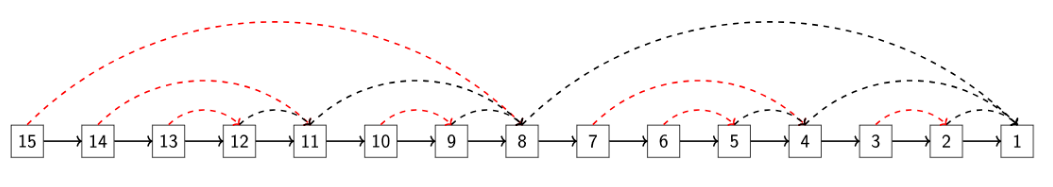
\includegraphics[width=0.48\linewidth]{Imagens/Basic-Lista}
    }
    \hfill
    \subfloat[Formato de árvore]{
        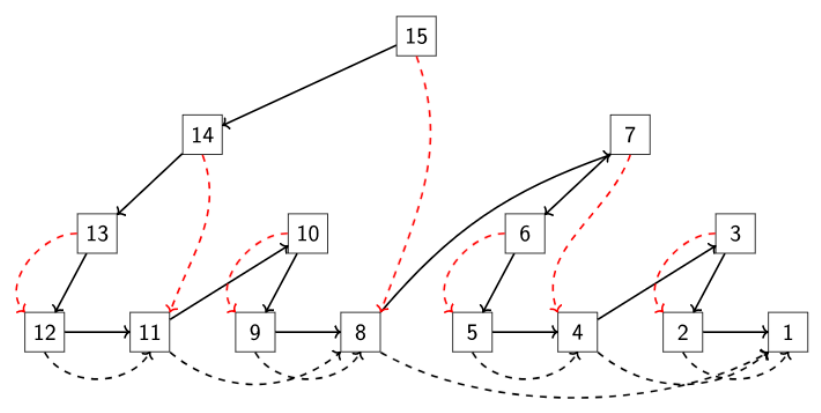
\includegraphics[width=0.4\linewidth]{Imagens/Basic-Arvore.png}
    }
    \caption{Representação da Basic Myers List}
    \label{fig:Basic}
\end{figure}

Assumindo as seguintes células, a associação do apontador \texttt{jump} para uma célula nova \(c\) funciona da seguinte forma:

\begin{figure}[H]
    \centering
    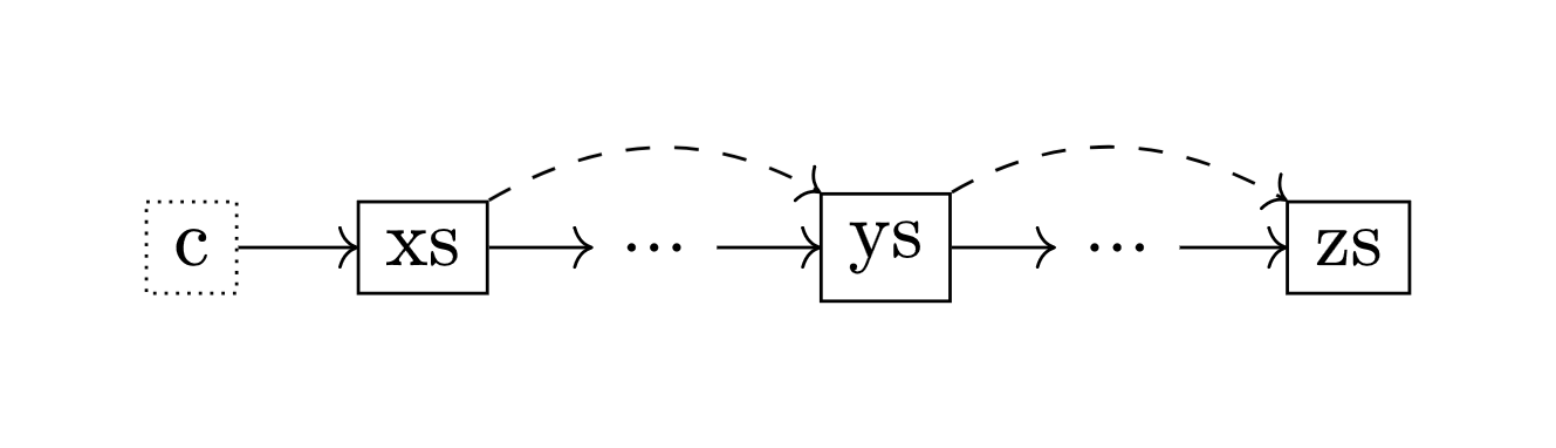
\includegraphics[width=0.5\linewidth]{Imagens/Basic-Cons}
    \caption{Exemplo de Basic Myers List, como células nomeadas}
    \label{fig:basic-cons}
\end{figure}

% Expressão matemática do jump
\begin{figure}[H]
    \centering
    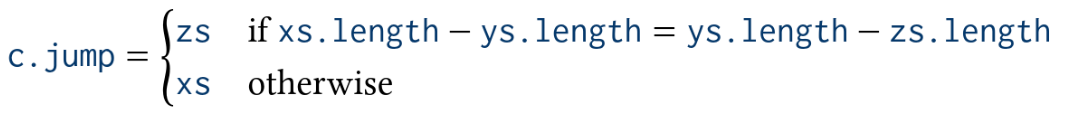
\includegraphics[width=0.5\linewidth]{Imagens/Basic-Jump} 
    \caption{\texttt{jump}}
    \label{fig:basic-jump}
\end{figure}

\textit{Lookup} na Basic Myers List é bastante simples, assume-se que \texttt{len} é um valor válido:

% Expressão matemática do lookup
\begin{figure}[H]
    \centering
    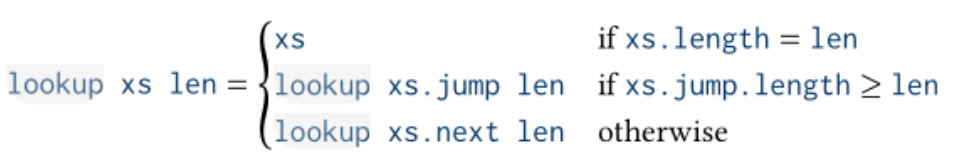
\includegraphics[width=0.5\linewidth]{Imagens/Basic-Lookup} 
    \caption{\textit{Lookup}}
    \label{fig:basic-lookup}
\end{figure}

\subsection{Improved Myers List}

A Improved Myers List, proposta por Peters, Foo e Adams (2025) \cite{peters2025}, introduz uma modificação simples, mas eficaz à maneira como a Basic Myers List é construída.
O apontador \texttt{jump} da primeira célula de cada região passa a apontar para a primeira célula da segunda sub-região, em vez da última 
célula. Assim, o resultado é uma melhoria do pior caso de \textit{lookup} de $3 \log(n) - 5$ para $2 \log(n + 1) - 3$ travessias, igualando ao desempenho da 
Okasaki List, estrutura de dados puramente funcional proposta por Chris Okasaki \cite{okasaki1995}, mas ainda com a vantagem de que permite o \textit{lookup} a partir de qualquer posição.

\begin{figure}[H]
    \centering
    
    \subfloat[Formato de lista]{
        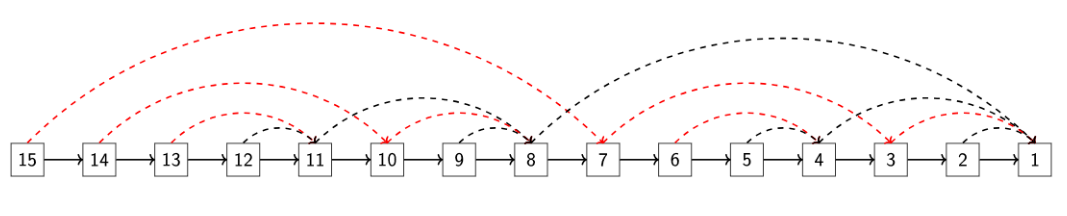
\includegraphics[width=0.48\linewidth]{Imagens/Improved-Lista}
    }
    \hfill
    \subfloat[Formato de árvore]{
        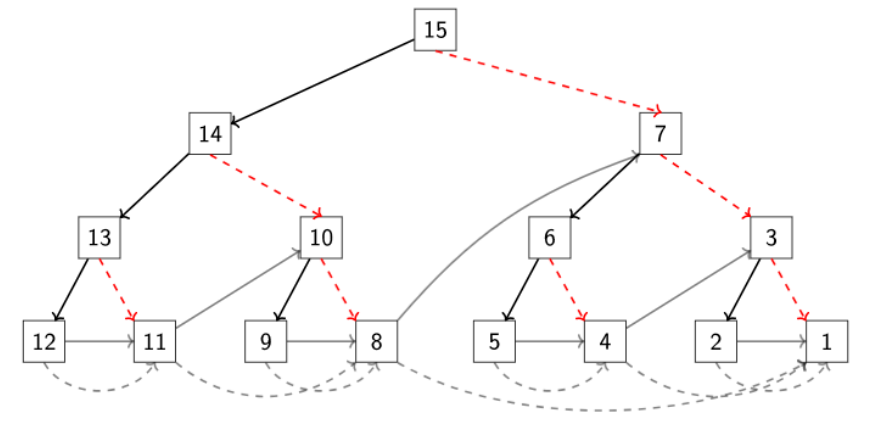
\includegraphics[width=0.4\linewidth]{Imagens/Improved-Arvore}
    }
    \caption{Representação da Improved Myers List}
    \label{fig:Improved}
\end{figure}


\subsubsection{Construção e conceito de região}

Uma região é definida pelo seu grau $k$:
\begin{itemize}
    \item Uma região de grau $k = 0$  consiste numa única célula.
    \item Uma região de grau $k > 0$ é composta por duas sub-regiões de grau $k - 1$ (no artigo, estas regiões são denominadas $Q_{k-1}$ e $R_{k-1}$) e uma célula adicional no início.
\end{itemize}

Na Basic Myers List, o apontador \texttt{jump} da célula inicial de uma região aponta para a última célula dessa mesma região. Adicionalmente, as duas 
sub-regiões partilham células, o que torna a estrutura menos eficiente.
A Improved Myers List resolve este problema alterando a regra de construção: as sub-regiões $Q_{k-1}$ e $R_{k-1}$ deixam de partilhar células, e o apontador 
\texttt{jump} da célula inicial passa a apontar diretamente para a primeira célula de $R_{k-1}$. Se visualizarmos a lista como uma árvore, as sub-regiões  $Q_{k-1}$ e 
$R_{k-1}$ formam, respetivamente, as sub-árvores esquerda e direita. Assim, o acesso à raiz da sub-árvore direita passa a custar apenas a travessia de 
um único apontador (\texttt{jump}), eliminando a ineficiência da variante clássica.

\begin{figure}[H]
    \centering
    \begin{tabular}{ccc}
        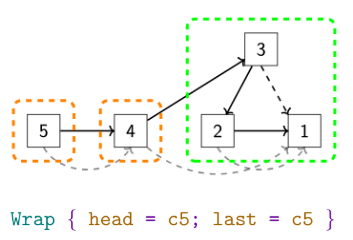
\includegraphics[width=0.3\linewidth]{Imagens/Regiao1} & 
        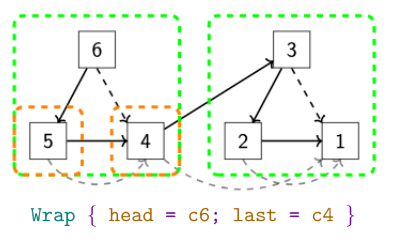
\includegraphics[width=0.3\linewidth]{Imagens/Regiao2} & 
        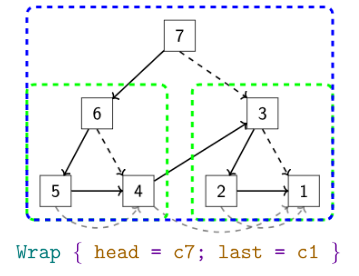
\includegraphics[width=0.3\linewidth]{Imagens/Regiao3}
    \end{tabular}
    \caption{Evolução do \texttt{wrap} durante o \textit{cons} na Improved Myers List}
    \label{tab:regioes}
\end{figure}

\subsubsection{\textit{Lookup}}

O algoritmo de \textit{lookup} na Improved Myers List é idêntico ao da Basic Myers List, percorre \texttt{jump} se \texttt{xs.jump.length} $\ge$ \texttt{len}, 
caso contrário, percorre \texttt{next}. 

\subsection{Advanced Myers List}

A Advanced Myers List, introduzida por Peters \cite{peters2025}, parte da Improved Myers List e introduz apontadores 
adicionais (\texttt{uncle}, \texttt{inc}, \texttt{greater}), permitindo assim um \textit{lookup} que pode ser realizado em tempo aproximadamente logarítmico 
$( 1 + \frac{1}{\sigma}) \log(n) + 9 + \sigma$ à custa de maior complexidade estrutural e de construção.


\begin{figure}[H]
    \centering
    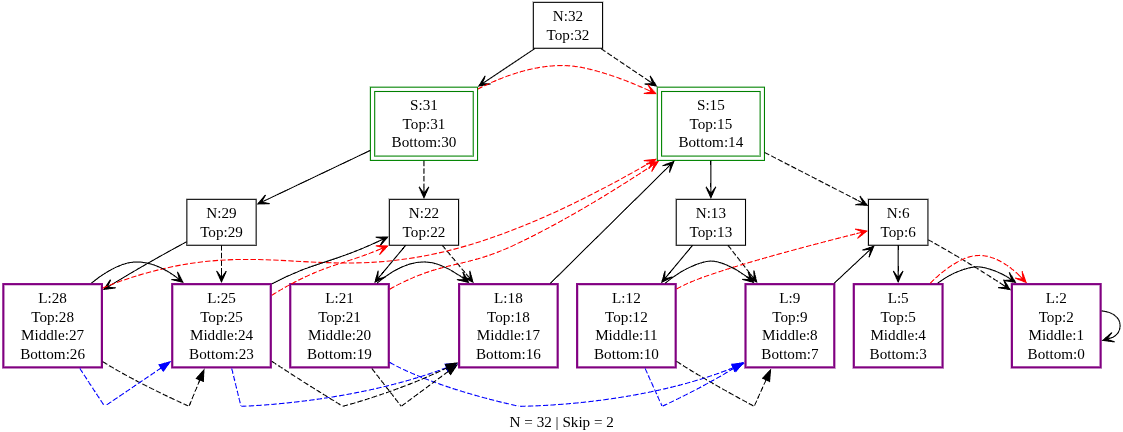
\includegraphics[width=0.8\linewidth]{Imagens/Advanced-Arvore} 
    \caption{Advanced Myers List}
    \label{fig:advanced}
\end{figure}

\subsubsection{Tipos de Nós}

A Advanced Myers List organiza as células em o que é chamado de nós lógicos, estes consistem em uma célula sozinha ou 
a junção de duas ou três células.
Existem três tipos de nós:
\begin{itemize}
    \item Nós normais -- são constituídos por apenas uma única célula (\textit{top}), contendo apontadores \texttt{next} e \texttt{jump} a apontar diretamente para os filhos esquerdo e direito.
    \item Nós \textit{skip} -- são constituídos por duas células, denominadas \textit{top} e \textit{bottom}. O apontador \texttt{next} da célula \textit{top} liga diretamente à célula bottom e o apontador \texttt{jump} aponta para o \texttt{uncle}. Estes nós aparecem repetidamente em camadas específicas, mais concretamente a cada intervalo \(\sigma\) acima da camada folha.
    \item Nós folha -- São constituídos pela junção de três células: \textit{top}, \textit{middle} e \textit{bottom}. Os apontadores \texttt{jump} de cada célula são reaproveitados para atalhos distintos: \texttt{inc}, \texttt{greater} e \texttt{uncle}. Estes nós constituem inteiramente a camada inferior da árvore lógica.
\end{itemize}


\begin{figure}[H]
    \centering
    \begin{tabular}{ccc}
        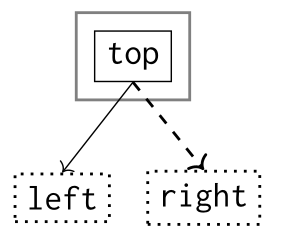
\includegraphics[width=0.2\linewidth]{Imagens/No-Normal} & 
        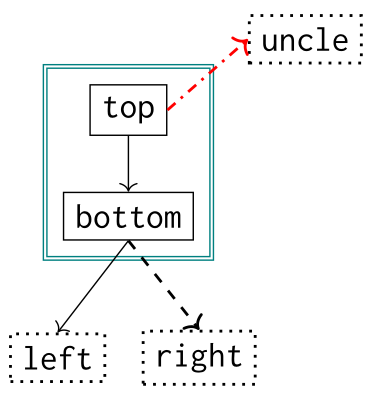
\includegraphics[width=0.2\linewidth]{Imagens/No-Skip} & 
        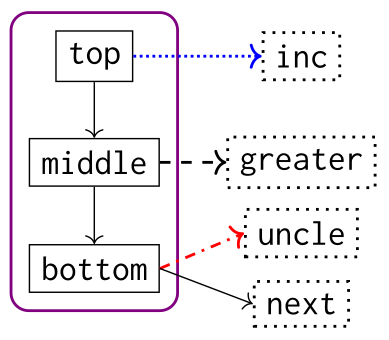
\includegraphics[width=0.2\linewidth]{Imagens/No-Leaf}\\
        Nós Normais & Nós \textit{Skip} & Nós Folha\\ 
    \end{tabular}
    \caption{Tipos de Nós}
    \label{tab:nos}
\end{figure}



\subsubsection{Construção}

Antes de discutir a construção é importante primeiro compreender os seguintes conceitos:
\begin{itemize}
    \item \textit{Right-Handed Depth} (RHD) -- Corresponde à distância do ancestral mais próximo que é um filho esquerdo.
    \item \textit{Right-Edge Depth} (RED) -- Corresponde à distância ao ancestral mais próximo que se encontra no caminho mais à direita a partir da raiz da árvore.
    \item \textit{Target uncle} -- Durante o algoritmo de \textit{lookup}, o \textit{target uncle} refere-se à criança direita do nó ancestral comum entre o nó de origem e o nó de destino.
\end{itemize}

A construção da Advanced Myers List perde a função de cons em tempo constante, pois exige saber previamente o número exato de elementos para calcular a altura da árvore lógica e formar uma árvore binária perfeita, utilizando elementos que servem como enchimento (\textit{fillers}) caso necessário.
A estrutura é construída recursivamente do \texttt{head} até a camada de folhas e a atribuição dos apontadores depende do tipo de nó:

\begin{itemize}
    \item Nós normais e \textit{skip}: O apontador \texttt{next} aponta para a sub-árvore esquerda e o \texttt{jump} para a sub-árvore direita
    \item Nós \textit{skip} e folhas: O apontador \texttt{uncle} liga a um tio onde a regra $\text{RED}(\texttt{s.uncle}) = \text{RHD}(\texttt{s})$ é verificada
    \item Nós folha: O apontador \texttt{inc} liga a uma folha mais próxima à direita tal que $\text{RHD}(f') = \text{RHD}(f) + 1$. O apontador \texttt{greater} liga à folha mais próxima à direita onde $\text{RHD}(f') > \text{RHD}(f)$, este apontador pode ser obtido recorrendo ao processo usado para o apontador \texttt{jump}.
\end{itemize}

\subsubsection{\textit{Lookup}}

O algoritmo de \textit{lookup} na Advanced Myers List determina dinamicamente o percurso ideal com base na posição relativa entre a célula de origem e a de destino, ramificando-se em três cenários fundamentais:

\begin{itemize}
    \item Descida Direta: Se o destino é um descendente direto da origem na árvore lógica, o algoritmo realiza uma descida através dos apontadores até alcançar o índice pretendido;
    \item Salto via \texttt{uncle}: Se existir um nó \textit{skip} ou folha descendente da origem cujo RHD coincida com o RED do \textit{target uncle}, o algoritmo salta diretamente para o \textit{target uncle} através do apontador \texttt{uncle};
    \item Travessia Lateral: Caso as condições de descendência não se apliquem, o algoritmo recorre aos apontadores \texttt{inc} para navegar horizontalmente entre nós folha adjacentes, ou ao apontador \texttt{greater} para saltar para a extremidade da subárvore corrente antes de transitar para a região seguinte da lista;
    \item Transição Ascendente: Quando nenhum dos três cenários anteriores é aplicável (por exemplo, quando a origem é uma folha cujo RHD já excede o RED necessário para o \textit{target uncle}), o algoritmo segue o apontador \texttt{next} para avançar para um nó não-folha. A partir dessa nova posição, é garantido que um dos três primeiros cenários será acionado.
\end{itemize}

\textbf{NOTA:} Aqui explicamos o funcionamento da Improved Myers List e da Advanced Myers List de uma forma muito superficial mas rápida de compreender, para uma compreensão e para um estudo mais informativo recomenda-se ler o artigo original.

\section{Estruturas Propostas}

\subsection{Dense Advanced Myers List} \label{subsec:dense_list}

A Dense Advanced trata-se de uma variação da Advanced Myers List criada por Peters \cite{peters2025}, mas em vez de dividir um nó com dois a quatro
apontadores, em um a três células, cada uma com dois apontadores. Decidimos representar cada nó com uma única célula, com o seu respetivo número de 
apontadores:

\begin{lstlisting} [style=ocaml_light, caption={Tipos de células}, captionpos=b, float=h]
type 'a add_points = 
    | Normal 
    | Skip of 'a cell 
    | Leaf of 'a cell * 'a cell
and 'a cell = { next : 'a cell; jump : 'a cell; length : int; 
    value : 'a; rhd : int; red : int; more : 'a add_points }
\end{lstlisting}

Isto tornou a implementação da estrutura mais fácil e por consequência, determinar o algoritmo para a operação \textit{cons} foi mais simples.
Outros benefícios desta alteração foram: Um número de travessias de apontadores menor; Encontraram-se novas otimizações que não foram ponderadas
na implementação original; E obteve-se um \textit{lookup} mais rápido.

No entanto, um defeito desta estrutura em relação à original, é que esta gasta mais memória, já que cada célula contém mais apontadores.

O caso uso mais apropriado para esta estrutura seria um ambiente onde a travessia de apontadores seria muito custosa, tal como referido para a 
lista original: «Thus, advanced Myers lists may not be appropriate for in-memory lists, but they may be useful for applications where the cost 
of pointer traversals is high relative to other computations, such as when pointer traversals involve network access.» (Peters et al., 2025, p. 13)


\begin{figure}[H]
    \centering
    
    \subfloat[Formato de lista]{
        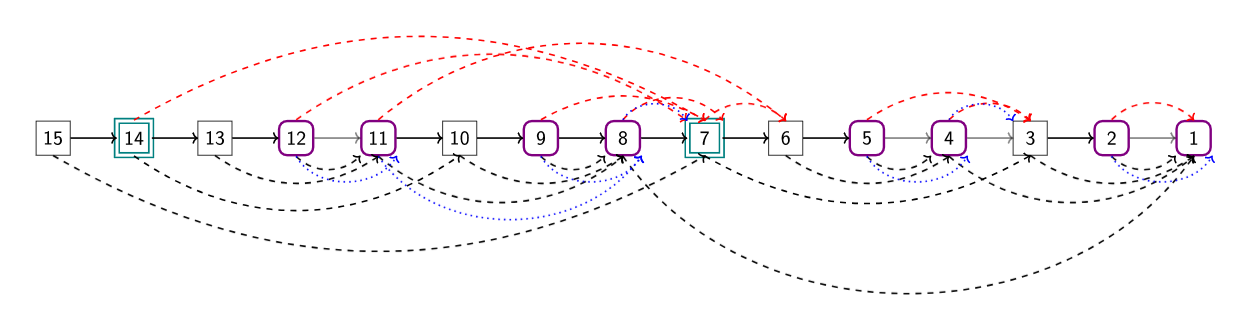
\includegraphics[width=0.48\linewidth]{Imagens/Dense-Lista}
    }
    \hfill
    \subfloat[Formato de árvore]{
        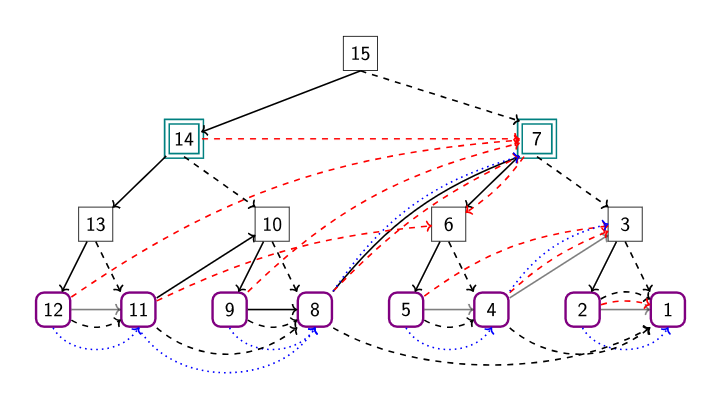
\includegraphics[width=0.48\linewidth]{Imagens/Dense-Arvore}
    }
    \caption{Representação da Dense Advanced Myers List}
    \label{fig:Dense}
\end{figure}


\subsubsection{\textit{Cons}}

Na Dense Advanced Myers List, o \textit{cons} difere das restantes variantes, uma vez que este não apresenta um \textit{cons} em tempo constante. 
A inserção de um novo elemento exige sempre o cálculo do RED e do RHD, além da atribuição dos apontadores \texttt{next} e \texttt{jump}. 
\\

O algoritmo determina o tipo de nó a ser criado com base na altura lógica e avaliando em relação ao $\sigma$. O motivo desta estrutura não 
apresentar um \textit{cons} em tempo constante deve-se a criação de novas células \textit{skip} (\texttt{Skip}) e folha (\texttt{Leaf}), estas células apresentam apontadores adicionais: \texttt{inc} e 
\texttt{uncle}. Que para receberem o valor apropriado é necessário atravessar a própria estrutura da lista à procura das células apropriadas com base 
nos valores do RED e RHD.


\subsubsection{\textit{Lookup}}

O algoritmo de \textit{lookup} na Dense Myers List é como uma busca hierárquica. Quando solicitamos o \textit{lookup} por um elemento em uma posição específica, 
o algoritmo primeiro calcula a distância que precisa para chegar ao alvo e avalia o tipo de nó atual, que pode ser uma célula do tipo normal, 
\textit{skip} ou folha. Se o destino estiver longe, o algoritmo usa os apontadores adicionais, \texttt{uncle} e \texttt{inc}. À medida que o algoritmo se aproxima do local 
desejado e a distância diminui, ele deixa de usar esses atalhos grandes e entra em uma etapa de descida. Nessa etapa final, ele faz saltos menores, 
\texttt{next} ou \texttt{jump}, até chegar com exatidão ao elemento procurado.


\subsection{Improved Applicative Random-Access Stack with Sigma region} \label{subsec:iarass}

A Improved Applicative Random-Access Stack with Sigma region (IARASS) é uma variante da Improved Myers List que se beneficia da introdução do 
conceito de \textit{sigma layers}, introduzido por Peters \cite{peters2025} na Advanced Myers List. Assim, o objetivo da IARASS é utilizar este novo apontador
para aliviar o problema da descida dupla (\textit{double descent}) identificado no artigo original, sem perder a simplicidade estrutural existente na variante Improved.
Na secção dos Resultados, mostraremos ainda que esta estrutura, como é de esperado, apresenta um maior uso de memória que a Improved Myers List, 
no entanto apresenta um menor uso de memória quando comparada com a Advanced Myers List e apresentando um maior desempenho no número de travessias 
quando comparada com ambas as variantes.
\\

Ao contrário da Improved Myers List em que todas as células apresentam a mesma estrutura, contendo os campos \texttt{next}, \texttt{jump}, \texttt{length} e \texttt{value}, a IARASS 
distingue dois tipos de células:

\begin{lstlisting} [style=ocaml_light, caption={Tipos de células}, captionpos=b]
type 'a cell = 
  | Normal of {next:'a cell; jump:'a cell; length:int; value:'a; height:int }
  | Skip of {next:'a cell; jump:'a cell; length:int; value:'a; height:int; shortcut:'a cell }
\end{lstlisting}

Nesta variante, as células normais mantêm apenas os dois apontadores já existente na variante Improved Myers List mantendo toda a lógica já existente, 
enquanto as células \textit{skip} (células de salto) apresentam um terceiro apontador, denominado \texttt{shortcut}. A decisão de qual célula é criada é baseada na altura (\texttt{height}). 

\begin{figure}[H]
    \centering
    
    \subfloat[Formato de lista]{
        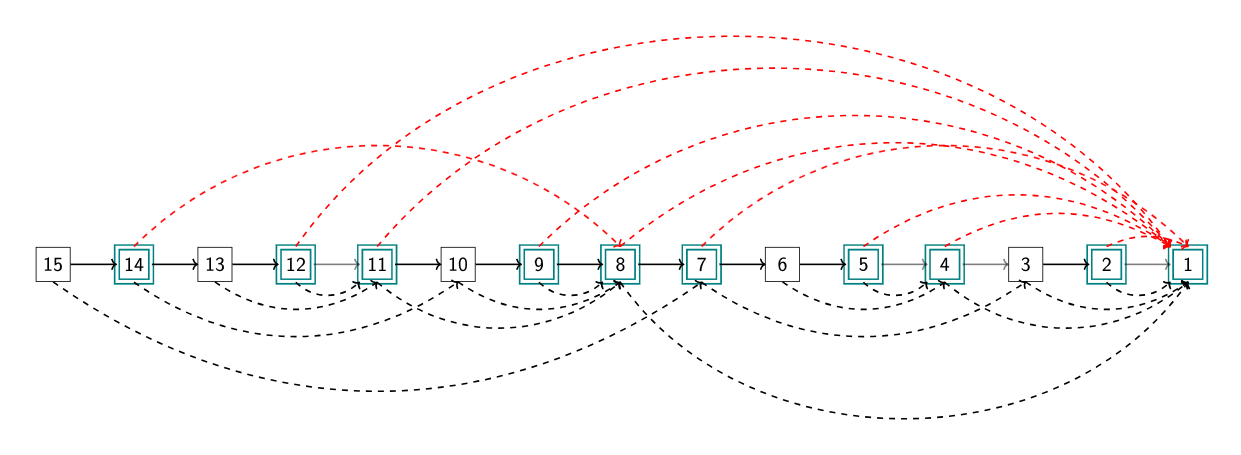
\includegraphics[width=0.48\linewidth]{Imagens/Iarass-Lista}
    }
    \hfill
    \subfloat[Formato de árvore]{
        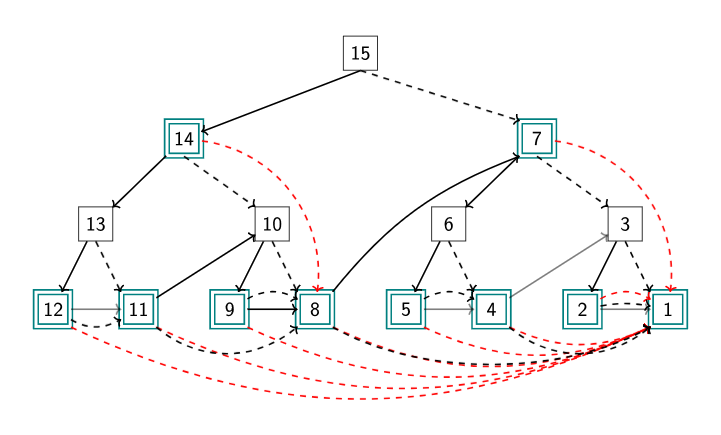
\includegraphics[width=0.4\linewidth]{Imagens/Iarass-Arvore.png}
    }
    \caption{Representação da IARASS}
    \label{fig:Iarass}
\end{figure}

\subsubsection{\textit{Cons}}

Durante a contrução de uma nova célula,
sempre que a altura é um divisor de $\sigma$, ou seja $\texttt{height} \bmod \sigma = 0$, a célula criada é do tipo \textit{skip} e nas restantes camadas serão do tipo normal. 
Ao contrário da Advanced Myers List, um $\sigma$ maior não indica uma melhor performance no \textit{lookup}, nesta estrutura a lógica é inversa, ou seja, quanto maior o $\sigma$ maior 
será o número de travessias, mas consequentemente usará menos memória.
\\

O novo apontador \texttt{shortcut} destas células \textit{skip} é a contribuição principal para resolver o problema da descida dupla e assume um comportamento diferente 
dependendo da posição da célula na árvore lógica: \textbf{(i)} quando a altura é diferente de 0, o \texttt{shortcut} aponta para a última célula da região que 
contém a célula acabada de ser criada. \textbf{(ii)} quando a altura é igual a 0, o \texttt{shortcut} aponta para \texttt{c.jump.jump.jump}, permitindo uma travessia horizontal 
mais rápida do que antes.  


\begin{comment}
A IARASS apresenta um \textit{cons} em tempo constante $\mathcal{O}(1)$ e apresenta um \textit{cons} muito semelhante a Improved Myers List, apenas diferenciando-se na ocasião dos nós 
\textit{skip}. Durante a inserção de um novo elemento, a altura lógica do novo nó a ser inserido é calculada, esta altura é utilizada para distinguir as 
células normais das células \textit{skip}. Sempre que a altura calculada for um divisor de $\sigma$, significa que a célula a ser criada é uma célula  \textit{skip}, caso 
contrário, a célula a ser criada é uma célula normal.

A atribuição do \texttt{shortcut} às células \textit{skip} difere dependendo da altura em que esta célula se encontra: \textbf{(i)} para alturas diferentes de 0, 
o \texttt{shortcut} aponta para o último elemento da região onde está inserida \textbf{(ii)} para alturas iguais a 0, o \texttt{shortcut} aponta para 3 saltos mais à frente, 
ou seja \texttt{get\_jump (get\_jump (get\_jump c))}.
\end{comment}

\subsubsection{\textit{Lookup}}

O algoritmo de \textit{lookup} na IARASS mantém-se idêntico à Improved Myers List nas células normais. Nas células \textit{skip}, o algoritmo verifica 
primeiro se é possível utilizar o \texttt{shortcut} para efetuar um salto maior, caso o \texttt{shortcut} ultrapasse a posição desejada, o algoritmo avalia o 
apontador \texttt{jump} e caso este também ultrapasse a posição desejada, optamos pela última opção de seguir pelo apontador \texttt{next}. 

\section{Resultados} \label{sec:resultados}

Nesta secção, apresentaremos os resultados obtidos na avaliação das cinco estruturas abordadas neste relatório, Basic, Improved e Advanced Myers List, Dense Advanced Myers List e IARASS. 

\newpage
\subsection{Número de Travessias}


Os gráficos da Tabela \ref{tab:travessias_1} e \ref{tab:travessias_2} comparam o número de travessias do pior caso com o limite 
teórico da estrutura, para listas de comprimento entre 1 e 1\_000\_000 elementos. 

% TODO: Fazer melhores gráficos e substituir 
\begin{table}[h!]
    \centering
    \begin{tabular}{cc}
         \includesvg[width=0.5\linewidth]{Imagens/3lgn.svg} & \includesvg[width=0.5\linewidth]{Imagens/2lgn.svg}\\ 
         (a) Basic Myers List & (b) Improved Myers List\\ 
         \includesvg[width=0.5\linewidth]{Imagens/1lgn-skip-2.svg} & \includesvg[width=0.5\linewidth]{Imagens/1lgn-skip-4.svg}\\
         (c) Advanced Myers List ($\sigma$ = 2) & (d) Advanced Myers List ($\sigma$ = 4)\\
         \includesvg[width=0.5\linewidth]{Imagens/1lgn-skip-8.svg} & \includesvg[width=0.5\linewidth]{Imagens/1lgn-skip-16.svg}\\
         (e) Advanced Myers List ($\sigma$ = 8) & (f) Advanced Myers List ($\sigma$ = 16)\\
    \end{tabular}
    \caption{Número de travessias - Basic, Improved e Advanced Myers List}
    \label{tab:travessias_1}
\end{table}


Os resultados confirmam a hierarquia Basic > Improved >= Advanced, mas mostram também que a escolha
de um sigma tem um impacto direto no ponto a partir do qual a Advanced Myers List compensa mais face 
à Improved Myers List. 

% TODO : Colocar o gráfico da Dense Advanced Myers List
% TODO : Centralizar o gráfico do Okasaki
\begin{table}[h!]
    \centering
    \begin{tabular}{cc}
         \includesvg[width=0.5\linewidth]{Imagens/3lgn.svg} & \includesvg[width=0.5\linewidth]{Imagens/iarass_1_000_000}\\
         (a) Dense Advanced Myers List & (b) Iarass\\
         \includesvg[width=0.5\linewidth]{Imagens/simon_cruanes_1_000_000.svg}\\
         (c) Okasaki List
    \end{tabular}
    \caption{Número de travessias - Dense Advanced Myers List, IARASS e Okasaki List}
    \label{tab:travessias_2}
\end{table}


A Tabela \ref{tab:pior_caso} apresenta o número máximo de travessias observado 
para n = 1 000 000, valores retirados da leitura visual dos gráficos 
anteriores com valores exatos para comparação direta entre estruturas.

% TODO: Expandir a parte da Advanced, ou seja, colocar uma linha por cada sigma
\begin{table}[h!]
    \centering
    \begin{tabular}{cc}
        \textbf{Variante} & \textbf{Pior caso registado} \\
        \hline
         Basic Myers List & 53\\
         \hline
         Improved Myers List & 35 \\
         \hline
         Advanced Myers List & [32, 41] (depende do sigma)\\
         \hline
         Dense Advanced Myers List (sigma = 2) & 24\\
         \hline
         Iarass & 27\\
         \hline
         Okasaki List & 37\\
         \hline
    \end{tabular}
    \caption{Pior caso de travessias registado (n = 1 000 000)}
    \label{tab:pior_caso}
\end{table}


\newpage
\subsection{Tempo de Execução}

A Tabela \ref{tab:tempo_execucao} apresenta o tempo total de execução de lookups sobre todos os elementos de uma lista 
com 1 000 000 de elementos para todas as variantes.

% TODO: Adicionamos mais alguma coluna?
\begin{table}[h!]
    \centering
    \begin{tabular}{cc}
        \textbf{Variante} & \textbf{Lookup All (1\_000\_000)} \\
        \hline
         Basic Myers List & 57.42 ms\\
         \hline
         Improved Myers List & 77.46 ms\\
         \hline
         Advanced Myers List & 401.43 ms\\
         \hline
         Dense Advanced Myers List (sigma = 2) & 60.35 ms\\
         \hline
         Iarass & 65.00 ms\\
         \hline
         Okasaki List & 51.04 ms\\
         \hline
    \end{tabular}
    \caption{Tempo de execução}
    \label{tab:tempo_execucao}
\end{table}


% TODO: Texto a explicar/falar dos dados obtidos

\newpage
\subsection{Uso de Memória}

A Tablea \ref{tab:memoria} apresenta o uso de memória de cada variante para uma lista de 1 000 000 de elementos.
Como era esperado, a Basic e a Improved Myers List apresentam exatamente o mesmo uso de memória 
(38.15 MB), uma vez que ambas mantêm o mesmo número de apontadores por célula, sendo apenas diferentes na maneira como o apontador jump é atribuído durante o cons.
\\
A Okasaki List  apresenta o menor uso de memória de todas as variantes (22.89 MB), por não incluir nenhum apontador adicional.

% TODO: continuar o texto e falar das restantes estruturas

\begin{table}[h!]
    \centering
    \begin{tabular}{cc}
        \textbf{Variante} & \textbf{Memória (1000000 elementos)} \\
        \hline
         Basic Myers List & 38.15 MB\\
         \hline
         Improved Myers List & 38.15 MB\\
         \hline
         Advanced Myers List & 53.41 MB\\
         \hline
         Dense Advanced Myers List (sigma = 2) & 75.02 MB\\
         \hline
         Iarass & 50.86 MB\\
         \hline
         Okasaki List & 22.89 MB\\
         \hline
    \end{tabular}
    \caption{Uso de memória para cada variante}
    \label{tab:memoria}
\end{table}
\section{Discussão}

A análise e avaliação das estruturas de dados desenvolvidas permitiu chegar a conclusões claras face as perguntas propostas nos objetivos.
Relativamente à primeira pergunta, a implementação da Dense Advanced Myers List concluiu que não foi possível obter uma operação cons em
tempo constante. Esta limitação deve-se à impossibilidade de aceder as células, que são utilizadas como ponteiro uncle,
greater ou inc, sem a necessidade de atravessar a lista ou fazer um lookup. No entanto, foi possível implementar uma operação cons funcional 
para esta estrutura, com uma complexidade temporal de [INSERIR A COMPLEXIDADE]. Importa destacar que o objetivo de um cons com tempo constante 
exige uma restruturação da arquitetura, objetivo para futuras investigações.

Apesar de o cons em O(1) não ter sido obtido, a Dense Advanced Myers List apresentou resultados eficazes na leitura, tendo um tempo de execução
de lookup total de 60,35 ms, valor muito inferior à variante Advanced Myers List com 401,43 ms. Além disso, ainda apresentou um melhoramento no 
número de travessias, obtendo o melhor desempenho no pior caso quando comparada a todas as outras estruturas. Este ganho de performance tem um 
custo direto associado à memória exigindo 75,02 MB para um milhão de elementos, sendo a estrutura mais pesada do nosso estudo. Assim, conclui-se 
que esta estrutura é ideal para cenários onde a travessia de ponteiros é o principal obstáculo.

Relativamente à segunda pergunta, a implementação da IARASS revelou ser um sucesso na diminuição do problema da dupla descida. Ao introduzir células 
skip com um apontador adicional, conseguimos reduzir o número de travessias no pior caso de 35 (variante Improved) para 27. Além disso, apresentou um 
tempo de execução de 65,00 ms, ultrapassando a Improved Myers List (77,46 ms) e a Advanced Myers List (401,43 ms). No que toca a uso de memória, a 
IARASS utiliza 50,86 MB, valor superior aos 38,15 MB da variante Improved e consumindo menos memória do que a Advanced Myers List (53,41 MB). 
Assim, conclui-se que esta estrutura apresenta um melhor desempenho global superior ao da Advanced Myers List, otimizando simultaneamente a velocidade
de execução, o número de travessias e a eficiência de memória.

Em suma, a remoção da restrição permitiu-nos implementar duas novas estruturas de dados com propostas de valor distintas.
A Dense Advanced Myers List é a melhor escolha quando a velocidade lookup é o mais importante e a memória não é um problema a ser considerado, 
continuando com a operação de cons. Por sua vez, a IARASS mostra ser uma estrutura de dados equilibrada que oferece melhorias consideráveis no 
desempenho de lookup com um aumento moderado na memória.
\section{Conclusão}

Em suma, a remoção da restrição permitiu-nos implementar duas novas estruturas de dados com propostas de valor distintas.
A Dense Advanced Myers List é a melhor escolha quando a velocidade \textit{lookup} é o mais importante e a memória não é um problema a ser considerado, 
continuando com a operação de \textit{cons}. Por sua vez, a IARASS mostra ser uma estrutura de dados equilibrada que oferece melhorias consideráveis no 
desempenho de \textit{lookup} com um aumento moderado na memória.

\input{Referencias}

\end{document}
